    \newcommand{\knnplot}[1]{
        \begin{tikzpicture}
            \begin{axis}[
                width=10cm,
                height=6cm,
                xmin=-0.2,
                xmax=1.2,
                ymin=-0.2,
                ymax=1.2,
                xmajorticks=false,
                ymajorticks=false,
                ylabel=y,
                xlabel=x,
                clip=false
            ]
                \ifnum#1=1
                    \addplot[
                        only marks,
                        opacity=0.5,
                        mark size=4pt
                    ] coordinates {
                        (0.000, -0.075)
                        (0.105, 0.075)
                        (0.211, 0.156)
                        (0.316, 0.295)
                        (0.421, 0.645)
                        (0.526, 0.685)
                        (0.684, 0.499)
                        (0.789, 0.602)
                        (0.895, 0.899)
                        (1.000, 1.140)
                    };
                \fi
                \ifnum#1>1
                    \ifnum#1<4
                        \addplot[
                            only marks,
                            opacity=0.1,
                            mark size=4pt
                        ] coordinates {
                            (0.000, -0.075)
                            (0.105, 0.075)
                            (0.211, 0.156)
                            (0.316, 0.295)
                            (0.421, 0.645)
                            (0.526, 0.685)
                            (0.684, 0.499)
                            (0.789, 0.602)
                            (0.895, 0.899)
                            (1.000, 1.140)
                        };
                        \draw[dashed] (axis cs: 0.6, -0.2) -- (axis cs: 0.6, 1.2);
                        \node[anchor=south] at (axis cs: 0.6, 1.2) {\small{?}};

                        \ifnum#1=3
                            \addplot[
                                only marks,
                                red,
                                mark size=4pt,
                                opacity=0.6
                            ] coordinates {
                                (0.6, 0.685)
                            };
                            \draw[-stealth,red] (axis cs: 0.60, 0.685) -- (axis cs: 0.55, 0.685);
                        \fi
                    \fi
                \fi

                \ifnum#1=4
                    \addplot[
                        only marks,
                        opacity=0.5,
                        mark size=4pt
                    ] coordinates {
                        (0.000, -0.075)
                        (0.105, 0.075)
                        (0.211, 0.156)
                        (0.316, 0.295)
                        (0.421, 0.645)
                        (0.526, 0.685)
                        (0.684, 0.499)
                        (0.789, 0.602)
                        (0.895, 0.899)
                        (1.000, 1.140)
                    };
                    \addplot[dashed] coordinates {
                        (-0.2, -0.075)
                        (0.0525, -0.075)
                        (0.0525, 0.075)
                        (0.1575, 0.075)
                        (0.1575, 0.156)
                        (0.263, 0.156)
                        (0.263, 0.295)
                        (0.368, 0.295)
                        (0.368, 0.645)
                        (0.473, 0.645)
                        (0.473, 0.685)
                        (0.578, 0.685)
                        (0.578, 0.499)
                        (0.7375, 0.499)
                        (0.7375, 0.602)
                        (0.842, 0.602)
                        (0.842, 0.899)
                        (0.9475, 0.899)
                        (0.9475, 1.140)
                        (1.2, 1.140)
                    };
                \fi

                \ifnum#1=5
                    \addplot[
                        only marks,
                        opacity=0.1,
                        mark size=4pt
                    ] coordinates {
                        (0.000, -0.075)
                        (0.105, 0.075)
                        (0.211, 0.156)
                        (0.316, 0.295)
                        (0.421, 0.645)
                        (0.526, 0.685)
                        (0.684, 0.499)
                        (0.789, 0.602)
                        (0.895, 0.899)
                        (1.000, 1.140)
                    };
                    \draw[dashed] (axis cs: 0.6, -0.2) -- (axis cs: 0.6, 1.2);
                    \node[anchor=south] at (axis cs: 0.6, 1.2) {\small{?}};
                    \addplot[
                        only marks,
                        red,
                        mark size=4pt,
                        opacity=0.6
                    ] coordinates {
                        (0.6, 0.592)
                    };
                    \draw[-stealth,red] (axis cs: 0.60, 0.592) -- (axis cs: 0.55, 0.66);
                    \draw[-stealth,red] (axis cs: 0.60, 0.592) -- (axis cs: 0.65, 0.52);
                \fi
                \ifnum#1=6
                    \addplot[
                        only marks,
                        opacity=0.5,
                        mark size=4pt
                    ] coordinates {
                        (0.000, -0.075)
                        (0.105, 0.075)
                        (0.211, 0.156)
                        (0.316, 0.295)
                        (0.421, 0.645)
                        (0.526, 0.685)
                        (0.684, 0.499)
                        (0.789, 0.602)
                        (0.895, 0.899)
                        (1.000, 1.140)
                    };
                    \addplot[dashed] coordinates {
                        (-0.2, 0)
                        (0.105, 0)
                        (0.105, 0.115)
                        (0.2105, 0.115)
                        (0.2105, 0.225)
                        (0.316, 0.225)
                        (0.316, 0.47)
                        (0.421, 0.47)
                        (0.421, 0.665)
                        (0.5525, 0.665)
                        (0.5525, 0.592)
                        (0.6575, 0.592)
                        (0.6575, 0.55)
                        (0.79, 0.55)
                        (0.79, 0.7505)
                        (0.894, 0.7505)
                        (0.894, 1.01)
                        (1.2, 1.01)


                    };
                \fi
                \ifnum#1=7
                \addplot[
                    only marks,
                    opacity=0.5,
                    mark size=4pt
                ] coordinates {
                    (0.000, -0.075)
                    (0.105, 0.075)
                    (0.211, 0.156)
                    (0.316, 0.295)
                    (0.421, 0.645)
                    (0.526, 0.685)
                    (0.684, 0.499)
                    (0.789, 0.602)
                    (0.895, 0.899)
                    (1.000, 1.140)
                };
                \addplot[dashed] coordinates {
                    (-0.2, 0.4921)
                    (1.2, 0.4921)
                };
            \fi

            \addplot[] coordinates {
                (-0.2, -0.2)
                (1.2, 1.2)
            };

            \end{axis}
        \end{tikzpicture}
    }

    \newsavebox{\knndata}
    \sbox{\knndata}{
        \knnplot{1}
    }
    \newsavebox{\knninput}
    \sbox{\knninput}{
        \knnplot{2}
    }
    \newsavebox{\knnpredone}
    \sbox{\knnpredone}{
        \knnplot{3}
    }
    \newsavebox{\knnformone}
    \sbox{\knnformone}{
        \knnplot{4}
    }
    \newsavebox{\knnpredtwo}
    \sbox{\knnpredtwo}{
        \knnplot{5}
    }
    \newsavebox{\knnformtwo}
    \sbox{\knnformtwo}{
        \knnplot{6}
    }
    \newsavebox{\knnall}
    \sbox{\knnall}{
        \knnplot{7}
    }

    \newcommand{\dimplot}[1]{
        \begin{tikzpicture}[scale=2]
            \node[] at (-1.5, -1.5) {};
            \node[] at (1.5, 1.5) {};

            \draw[-stealth,gray!50] (-1, -1) -- (1, -1);
            \node[anchor=north,,gray!50] at (0, -1) {$x_1$};
            \node[
                inner sep=2pt,
                circle,
                draw=black,
                fill=teal!60
            ] (n1) at (-0.8, -0.8) {};

            \ifnum#1=1
                \node[
                    inner sep=2pt,
                    circle,
                    draw=black,
                    fill=teal!60
                ] (n2) at (0.2, -0.8) {};
                \draw[dashed,stealth-stealth] (-0.75, -0.8) -- (0.15, -0.8) node [midway, above] {\small{1}};
            \fi

            \ifnum#1>1
                \draw[-stealth,gray!50] (-1, -1) -- (-1, 1);
                \node[anchor=east,gray!50] at (-1, 0) {$x_2$};
            \fi

            \ifnum#1=2
                \node[
                    inner sep=2pt,
                    circle,
                    draw=black,
                    fill=teal!60
                ] (n2) at (0.2, 0.2) {};
                \draw[dashed,stealth-] (-0.75, -0.8) -- (0.2, -0.8) node [midway, above] {\small{1}};
                \draw[dashed,-stealth] (0.2, -0.8) -- (0.2, 0.15) node [midway, right] {\small{1}};
                \draw[-stealth,red] (n1) -- (n2) node [pos=0.45, above=0.15cm] {\small{$\sqrt{2}$}};
            \fi

            \ifnum#1=3
                \draw[-stealth,gray!50] (-1, -1) -- (0.5, 0.0);
                \node[anchor=north, rotate=30,gray!50] at (-0.25, -0.5) {$x_3$};
                \node[
                    inner sep=2pt,
                    circle,
                    draw=black,
                    fill=teal!60
                ] (n2) at (0.7, 0.53) {};
                \draw[dashed,stealth-] (-0.75, -0.8) -- (0.2, -0.8) node [midway, above] {\small{1}};
                \draw[dashed,-stealth] (0.2, -0.8) -- (0.2, 0.2) node [midway, right] {\small{1}};
                \draw[dashed,-stealth] (0.2, 0.2) -- (0.7, 0.53) node [pos=0.4, below=0.15cm] {\small{1}};
                \draw[-stealth,red] (n1) -- (n2) node [pos=0.45, above=0.15cm] {\small{$\sqrt{3}$}};
            \fi

        \end{tikzpicture}
    }

    \newsavebox{\dimone}
    \sbox{\dimone}{
        \dimplot{1}
    }
    \newsavebox{\dimtwo}
    \sbox{\dimtwo}{
        \dimplot{2}
    }
    \newsavebox{\dimthree}
    \sbox{\dimthree}{
        \dimplot{3}
    }

    \section{K-Nearest Neighbours}

    \begin{frame}{K-Nearest Neighbours}
        \only<1-17>{
            \begin{tikzpicture}
                \node[] at (-5.25, -3) {};
                \node[] at (5.25, 3) {};

                \only<1-6>{
                    \node[align=center] at (0, 1) {
                        \textbf{Linear regression:}\\
                        $\hat{f}(X)=\alert<2>{\beta_0}+\alert<2>{\beta_1}X_1+\alert<2>{\beta_2}X_2+\ldots+\alert<2>{\beta_p}X_p$
                    };
                }
                \only<3-6>{
                    \node[align=center] at (0, -1) {
                        \textbf{K-Nearest Neighbours:}\\
                        $\hat{f}(X)=\frac{1}{\alert<6>{K}}\sum\limits_{\alert<4>{x_i \in \mathcal{N}}}\alert<5>{y_i}$
                    };
                }
                \only<7>{
                    \node[anchor=south west] at (-4.75, -2.5) {
                        \usebox{\knndata}
                    };
                }
                \only<8>{
                    \node[anchor=south west] at (-4.75, -2.5) {
                        \usebox{\knninput}
                    };
                }
                \only<9>{
                    \node[anchor=south west] at (-4.75, -2.5) {
                        \usebox{\knnpredone}
                    };
                }
                \only<10>{
                    \node[anchor=south west] at (-4.75, -2.5) {
                        \usebox{\knnformone}
                    };
                }
                \only<11>{
                    \node[anchor=south west] at (-4.75, -2.5) {
                        \usebox{\knnpredtwo}
                    };
                }
                \only<12>{
                    \node[anchor=south west] at (-4.75, -2.5) {
                        \usebox{\knnformtwo}
                    };
                }
                \only<13>{
                    \node[anchor=south west] at (-4.75, -2.5) {
                        \usebox{\knnall}
                    };
                }
                \only<14>{
                    \node[align=left] at (0, 0) {
                        How does the bias-variance trade-off relate to the choice of $K$?
                    };
                };
                \only<15>{
                    \node[align=center] at (0, 0) {
                        \textbf{The curse of dimensionality:}\\
                        Things become complicated in very high dimensions
                    };
                };
                \only<16>{
                    \node[] at (0, 0) {
                        \usebox{\dimone}
                    };
                }
                \only<17>{
                    \node[] at (0, 0) {
                        \usebox{\dimtwo}
                    };
                }
                \only<18>{
                    \node[] at (0, 0) {
                        \usebox{\dimthree}
                    };
                }
            \end{tikzpicture}
        }
        \only<18>{
            \textbf{K-Nearest Neighbours: An intuitive model relying on similarities between datapoints to make predictions}
            \begin{itemize}
                \item No assumptions about the functional relationship between inputs and outputs
                \item Directly trades off bias and variance through the choice of $K$
                \item Does not work well in high dimensions as space gets more sparsely populated, yielding less dense neighbourhoods
                \item \textbf{Can be fidgety in practice (e.g. how should one choose the scales of different predictors), not very commonly used}
            \end{itemize}
        }
    \end{frame}

    \newcommand{\logisticplot}[1]{
        \begin{tikzpicture}
            \begin{axis}[
                height=5cm,
                width=10cm,
                ytick={0, 1},
                ytick style={draw=none},
                xtick pos=bottom,
                xlabel=x (mpg),
                ylabel=y (chevrolet),
                ymin=-0.5,
                ymax=1.5,
                xmin=13,
                xmax=38
            ]
                \addplot[
                    only marks,
                    fill=red,
                    mark size=3pt
                ] coordinates {
                    (36, 1)
                    (25, 1)
                    (26, 1)
                    (32, 1)
                    (28, 1)
                    (29, 1)
                    (29.5, 1)
                    (21, 1)
                };
                \addplot[
                    only marks,
                    fill=blue,
                    mark size=3pt
                ] coordinates {
                    (15, 0)
                    (17, 0)
                    (21, 0)
                    (14, 0)
                    (14.5, 0)
                    (16, 0)
                    (19, 0)
                    (24, 0)
                    (27, 0)
                };

                \ifnum#1=2
                    \addplot[
                        domain=10:40,
                        samples=100,
                        color=red,
                        thick
                    ] {-0.87+0.06*x};
                \fi
                \ifnum#1=3
                    \draw[dashed] (axis cs: 25.5, -0.5) -- (axis cs: 25.5, 1.5);
                    \draw[] (axis cs: 25.5, 1) -- (axis cs: 38, 1);
                    \draw[] (axis cs: 25.5, 0) -- (axis cs: 13, 0);
                \fi
                \ifnum#1=4
                    \addplot[
                        domain=13:38,
                        samples=100,
                        color=red,
                        thick
                    ] {exp(-10+0.42*x)/(1+exp(-10+0.42*x))};

                \fi
            \end{axis}
        \end{tikzpicture}
    }

    \newsavebox{\logisticdata}
    \sbox{\logisticdata}{
        \logisticplot{1}
    }
    \newsavebox{\logisticlinear}
    \sbox{\logisticlinear}{
        \logisticplot{2}
    }
    \newsavebox{\logisticstep}
    \sbox{\logisticstep}{
        \logisticplot{3}
    }
    \newsavebox{\logisticlog}
    \sbox{\logisticlog}{
        \logisticplot{4}
    }

    \section{Logistic regression}

    \begin{frame}{Logistic regression}
        \only<1-20>{
            
\begin{tikzpicture}
                \node[draw=black] at (-5.25, -4) {};
                \node[draw=black] at (5.25, 3) {};

                \only<1-2>{
                    \node[] at (0, 0) {
                        \begin{tabular}{ccc}
                            \textbf{mpg}&\textbf{manufacturer}&\textbf{chevrolet}\\
                            36&Chevrolet&1\\
                            15&Ford&0\\
                            25&Chevrolet&1\\
                            26&Chevrolet&1\\
                            17&Ford&0\\
                            15&Ford&0\\
                            32&Chevrolet&1\\
                            14&Ford&0\\
                            14&Ford&0\\
                            28&Chevrolet&1\\
                        \end{tabular}
                    };
                }
                \only<1>{
                    \node[] at (0, -3.5) {
                        $\widehat{\text{mpg}}=\beta_0+\beta_1\times\text{chevrolet}$
                    };
                }
                \only<2>{
                    \node[] at (0, -3.5) {
                        $\widehat{\text{chevrolet}}=\beta_0+\beta_1\times\text{mpg}$
                    };
                }
                \only<3>{
                    \node[] at (0, 0) {
                        \usebox{\logisticdata}
                    };
                }
                \only<4>{
                    \node[] at (0, 0) {
                        \usebox{\logisticlinear}
                    };
                    \node[] at (0, -3) {
                        $\widehat{\text{chevrolet}}=-0.87+0.06\times\text{mpg}$
                    };
                }
                \only<5>{
                    \node[] at (0, 0) {
                        \usebox{\logisticstep}
                    };
                }
                \only<6>{
                    \node[] at (0, 0) {
                        \usebox{\logisticlog}
                    };
                    \node[] at (0, -3) {
                        $\widehat{\text{chevrolet}}=\dfrac{e^{-10.22+0.42\times\text{mpg}}}{1 + e^{-10.22+0.42\times\text{mpg}}}$
                    };
                }
                \only<7-20>{
                    \node[] at (0, 1) {
                        $\hat{y}=\dfrac{e^{\beta_0+\beta_1x}}{1+e^{\beta_0+\beta_1x}}$
                    };
                }
                \only<8-13>{
                    \node[anchor=east] at (0, -1) {
                        $e^{\beta_0+\beta_1x} \rightarrow 0$
                    };
                }
                \only<9-13>{
                    \node[anchor=west] at (0, -1) {
                        $\implies \hat{y} = 0$
                    };
                }
                \only<10-13>{
                    \node[anchor=east] at (0, -1.5) {
                        $e^{\beta_0+\beta_1x} \rightarrow \infty$
                    };
                }
                \only<11-13>{
                    \node[anchor=west] at (0, -1.5) {
                        $\implies \hat{y} = 1$
                    };
                }
                \only<12-13>{
                    \node[anchor=east] at (0, -2.5) {
                        $0\leq\hat{y}\leq1$
                    };
                }
                \only<13>{
                    \node[anchor=west] at (0, -2.5) {
                        $\implies\hat{y}=Pr(Y=1|X)$
                    };
                }
                \only<15-16>{
                    \node[] at (0, -1) {
                        $log \left( \dfrac{p(X)}{1-p(X)} \right) = \beta_0+\beta_1x$
                    };
                }
                \only<16>{
                    \node[] at (0, -3) {
                        "\textit{... counterintuitive and challenging to interpret.}" - James Jaccard
                    };
                }
                \only<18-20>{
                    \node[] at (0, 0) {
                        More than one class?
                    };
                }
                \only<19-20>{
                    \node[] at (0, -2) {
                        $Pr(Y=k|X=x)=\dfrac{e^{\beta_{0k}+\beta_{1k}x}}{\sum\limits_{l=1}^{K}e^{\beta_{0l}+\beta_{1l}x}}$
                    };
                }
                \only<20>{
                    \node[rotate=45, fill=white, draw=black] at (0, 0) {
                        \Huge{Blackboard!}
                    };
                }
            \end{tikzpicture}
        }
        \only<21>{
            \textbf{Logistic regression: Extends linear regression to classification.}
            \begin{itemize}
                \item Treats all members of a class (approximately) equally.
                \item Ouputs an understandable quantity: The probability of a sample belonging to the positive class.
                \item Somewhat interpretable, although not as much as linear regression
                \item Can trivially be extended to include multiple classes
            \end{itemize}
        }
        \only<22>{
            \scriptsize{\url{http://localhost:8888/notebooks/notebooks\%2FLogistic\%20regression.ipynb}}
        }
    \end{frame}

    \section{Classification metrics}

    \begin{frame}{Classification metrics}
        The two most common, severe, mistakes made in machine learning studies in psychology and neuroscience (in my opinion) are:
        \begin{itemize}
            \item Poor validation and testing strategies (Lecture 4)
            \item Using incorrect performance measures, most commonly accuracy (Blackboard!)
        \end{itemize}
    \end{frame}
